\chapter{Communication Protocol}

This section describes the communication protocol used for command and data exchange between bus participants. Further, the bus monitor module, which is part of the \gls{FBU} is explained.

\section{Protocol}
\label{sec:protocol}

In initial system designs the usage of the CAN protocol was intended. This approach was discarded, because no license for the Xilinx CAN IP core could be obtained. Since no stable open source CAN IP core was found, a new protocol was defined.

In our approach a simple master-slave protocol was defined to enable communication between the master (\gls{ECU}, \gls{FBU}) and the slaves (\gls{THS}, \gls{MCU}, \gls{FBU}).
The protocol consists of command and data packets, each of them contains just one byte.
No error protection measures were taken into account.
Each bus participant needs a unique address. Since this design just contains three control units, two bits as address field are sufficient. Figure \ref{fig:Protocol} shows the composition of a control and data packets.

\begin{figure}[h!]
    \centering
    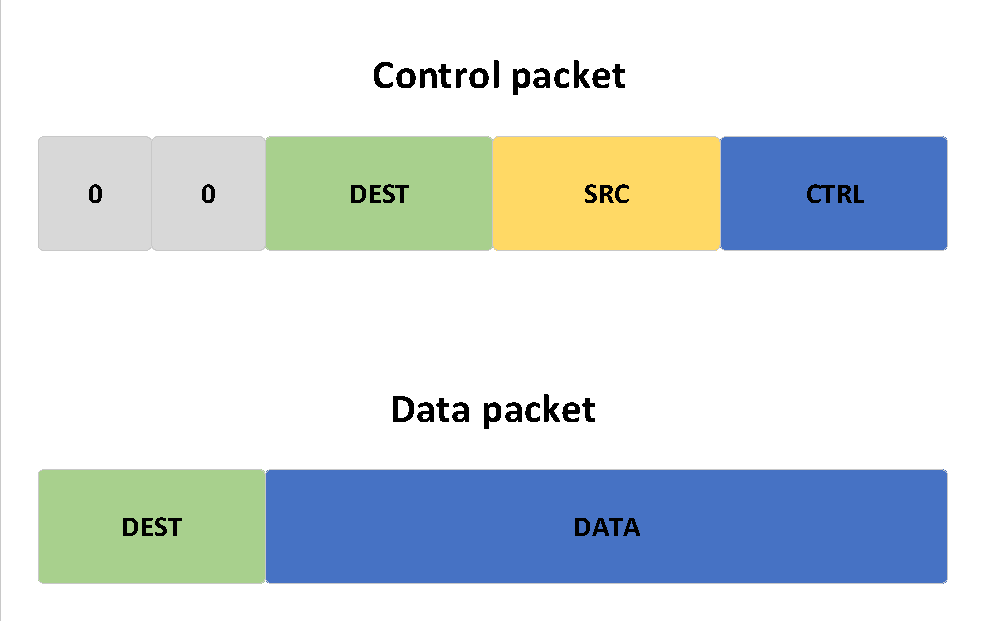
\includegraphics[width=0.75\textwidth]{figures/Protocol.pdf}
    \caption{Composition of control and data packets}\label{fig:Protocol}
\end{figure}

A control packet is indicated by two leading zeroes, followed by destination address (DEST) and source address (SRC). The last two bits (CTRL) determine a further classification of the control packet, as shown in table \ref{tab:controlPacket}.

\begin{table}[h!]
\begin{center}
\begin{tabular}{|c|c|c|}
\hline
\multicolumn{2}{|c|}{\textbf{CTRL}}&\textbf{Function} \\
\hline
0 & 0 & Request data \\
\hline
0 & 1 & Acknowledge \\
\hline
1 & 0 & Error 1 \\
\hline
1 & 1 & Error 2 \\
\hline
\end{tabular}
\end{center}
\caption{Control packet classification}
\label{tab:controlPacket}
\end{table}

A control packet can be used to request data, send an acknowledge or indicate errors. Only the master is able to send a request data command, the remaining control packet classifications can be used by the slaves, too.

A data packet starts with the destination address (DEST), followed by a 6 bit wide data field (DATA). It can be sent by the master and by slaves (if a request data command was received previously). If sent by a master, the slave has to answer with an acknowledge.

Since no measures to detect or correct data transmission errors are used, a sending retry mechanism is implemented. If the master doesn't receive an answer from a slave, it re-sends the packet up to a configurable number of attempts.

\section{Bus monitor}

The bus monitor module is part of the \gls{FBU} and is responsible for monitoring the traffic on the communication link to detect faulty units. Therefore it has to implement the protocol described in section \ref{sec:protocol}. 
The bus monitor is implemented as VHDL module and is implemented in the static area of the \gls{FPGA}. It detects the following incidents:

\begin{itemize}
    \item Timeout occurence
    \item Faulty packets
	\begin{itemize}
    		\item Wrong address
   		\item Error flag set (CTRL field)
	\end{itemize}
\end{itemize}

Seperate timeouts are configurable for master and slaves. The bus monitor also implements the retry mechanism according to section \ref{sec:protocol}.

The interfaces between the bus monitor, the reconfiguration controller and the bus is shown in figure \ref{fig:BusMonitor}.

\begin{figure}[h!]
    \centering
    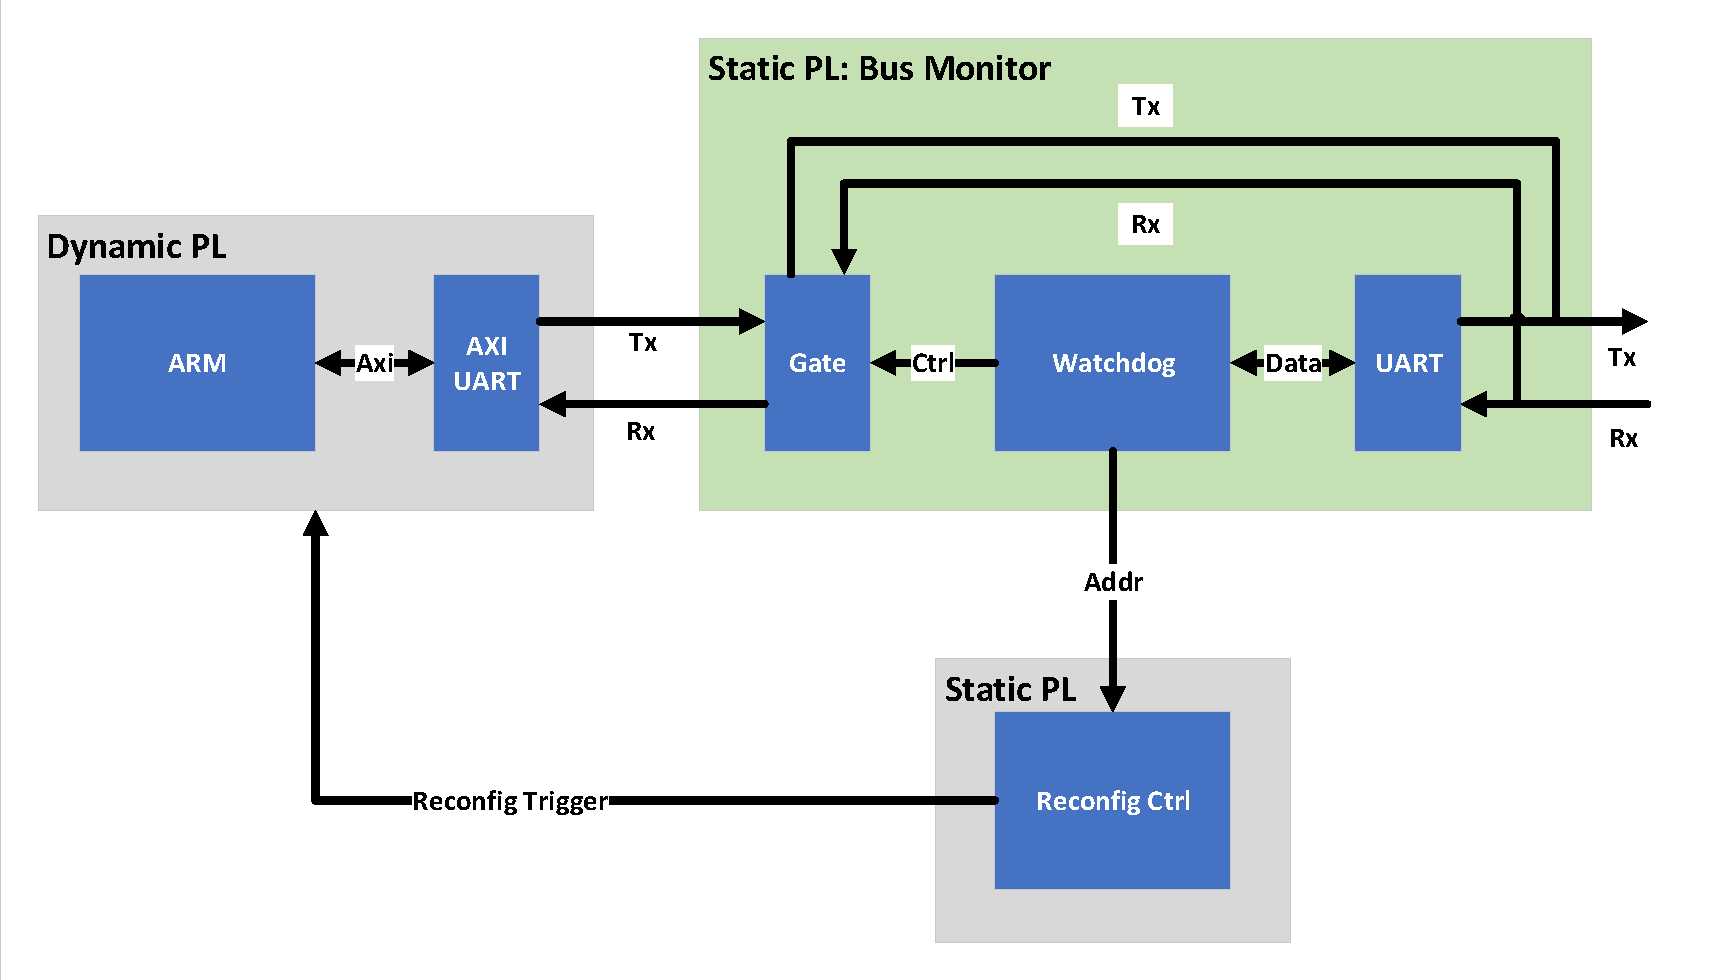
\includegraphics[width=\textwidth]{figures/BusMonitor.pdf}
    \caption{Bus monitor interfacing}\label{fig:BusMonitor}
\end{figure}

Since the system uses UART as physical communication layer (see section \ref{}), the UART IP (Martin Mosbeck) is used to retrieve data from the bus, which is forwarded to the watchdog unit within the bus monitor module. The watchdog is responsible for error and timeout detection. 
In case of an error or timeout detection, the address of the faulty unit is passed to the reconfiguration controller (using one-hot coding) to trigger a \gls{PR}. 
A gate circuit is used to pass the \gls{UART} receive (Rx) and transmit (Tx) line to the dynamic area once a reconfiguration was triggered. This is a safety measure to just allow transmission by the \gls{FBU} if a faulty unit has to be replaced. 
It is assumed, that just one bus participant can be replaced by the \gls{FBU} during system runtime, so once a reconfiguration was done, the bus monitoring is stopped.

The bus monitor is also used to control output pins of the \gls{FBU} if no bus participant has to be replaced, or if a bus participant that doesn't require any output pins is replaced. 
This is necessary, because the \gls{FPGA} which is used in this test setup pulls (unconfigured) output pins to low, which is not acceptable in our system (see section \ref{}).
